\chapter{Phase Diversity}
\label{ch:PDThe}

The phase diversity was first implemented by R. A. Gonsalves in 1976 \citep{Gonsalves_1976,Gonsalves_1982} to retrieve the phase of a wavefront coming from a point source. It uses two images, one at the focal plane and another one with a diversity introduced, such as defocus, in order to recover the phase of the wavefront. This chapter introduce the principle on which the phase diversity is based and then describes its implementation with two different algorithms. The first one is an algorithm developed at the ONERA by \citet{mugnier_2006}. The second algorithm presented is the one we developed in the frame of this study, which is based on an analytical approach developed by Dr. Laurent Jolissaint and refine by Jordan Voirin.

\section{Principle}
\label{sec:principle}

\begin{figure}
\begin{center}
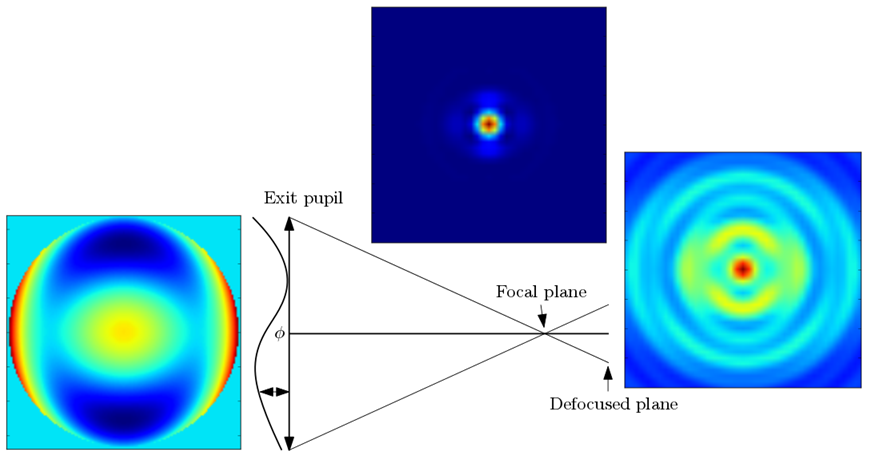
\includegraphics[width=0.8\textwidth,angle=0]{Figures/DiversityPrincipleM}
\decoRule
\caption{Schema of the phase diversity principle. The images from left to right are : the phase arriving on the exit pupil, the focused image and the defocused ($2\pi$) image.}
\label{fig:DiversityPrinciple}
\end{center}
\end{figure}

Unlike Shack-Hartmann wavefront reconstruction, which is a pupil plane technique, the phase diversity uses data acquired at the focal plane. Using the non-linear relation between the phase of the wavefront and the image, 

\begin{equation}
i(x,y) = (h_{optical}\otimes o)(x,y), \ with \ h_{optical}(x,y) = |\left[\mathcal{F}\left\lbrace A(\xi,\eta)e^{j\phi(\xi,\eta)} \right\rbrace\right](x,y)|^2,
\label{eqt:img-hopt}
\end{equation}

one can determine the phase, i.e. the aberrations present in the imaging system, by solving an inverse problem. The major difficulty of this technique is that, as one can see in eqt. \eqref{eqt:img-hopt}, there is not a unique solution to the problem at hand. This indetermination comes from the fact that the available detector can only sense the intensity of the wave, and not the wave itself, which is the modulus squared of the complex amplitude as exposed in section \ref{sec:ImSystem}. Thus, $\phi(\xi,\eta)$ and $\phi'(\xi,\eta)=-\phi(-\xi,-\eta)$ give the same PSF.
More specifically by decomposing the phase in its even and odd part and using the autocorrelation properties ($\Gamma_A = \Gamma_{A'}$ with $A'(t) = A*(-t)$), with only one image, one can not determine the sign of the phase even part. This leads to the introduction of a phase diversity to raise the indetermination. The idea is to add a known aberration $\delta\phi$ to the system and to use the two images to retrieve the phase of the wavefront.

The diversity between the two images is introduced for instance by defocusing one of the two images. In this work we will use this diversity, but having a more complex system, such has a deformable mirror, one could introduce any other even aberration such as an astigmatism, the only requirement is that the diversity introduced must have an even radial and azimuthal order. Figure \ref{fig:DiversityPrinciple} shows the principle of the phase diversity. Two images are acquired, one at the focal plane and another with a defocus. In this work, we introduce the defocus by sliding the detector along the z-axis, others use a beamsplitter and another detector \citep{mugnier_2006}.

The phase diversity is a technique that is sensible to chromatism, since it is based on diffraction. The non-linear relation that links the image and the phase depends also on the object. This renders the inverse problem to solve more complicated, but it allows to retrieve the phase, the object or both, when the object is unknown (most of the time). Furthermore, it is very simple optically, do not require a complex optical components to acquire the data, one just uses the detector in place. And it depends directly on the images so there is no noncommon-path aberration between the adaptive optic system and the scientific detector.

In this work, the final application of the phase diversity algorithm will be to correct for static aberration in an optical system. We will have knowledge of the object, since it will be a point source that we introduce with a laser or choose in the sky (a star).

\section[ONERA algorithm]{ONERA algorithm, \citet{mugnier_2006}}
\label{sec:ONERAalgo}

In this section, we will briefly present the phase diversity algorithm developed at ONERA since we test and use it to retrieve the phase and the aberrations in the experiment conducted in laboratory.

\subsection{Algorithm description}
\label{subsec:OneraAlgoDesc}

As explained in section \ref{sec:principle}, the phase diversity determines the phase of the wavefront, as well as the unknown object when needed, using two images of the same object with a phase diversity between each image. This gives the following equation system \citep[p.11]{mugnier_2006},

\begin{align}
\mathbf{i}_f &= \mathbf{h}_f \ast \mathbf{o} + \mathbf{n}_f \\
\mathbf{i}_d &= \mathbf{h}_d \ast \mathbf{o} + \mathbf{n}_d,
\label{eqt:systemEQT}
\end{align}

where the bold letters means that it is the sampled quantities, the indexes f and d means respectively focused and defocused and $\mathbf{n}$ regroups the photon and detector noise present on the image. Using the data available, this algorithm approaches the problem at hand with a statistic point of view. They estimate jointly the aberrations and the object \citep{Paxman1992}, which consist to compute the joint maximum \textit{a posteriori} (JMAP) estimator \citep[p.17]{mugnier_2006},

\begin{align}
(\hat{\mathbf{o}},\hat{\boldsymbol{\phi}})_{MAP} &= \underset{\mathbf{o},\boldsymbol{\phi}}{\mathrm{arg \ max}} \ p(\mathbf{i}_f,\mathbf{i}_d,\mathbf{o},\boldsymbol{\phi};\boldsymbol{\theta})\nonumber \\
&= \underset{\mathbf{o},\boldsymbol{\phi}}{\mathrm{arg \ max}} \ p(\mathbf{i}_f|\mathbf{o},\boldsymbol{\phi};\boldsymbol{\theta_n})p(\mathbf{i}_d|\mathbf{o},\boldsymbol{\phi};\boldsymbol{\theta_n})p(\mathbf{o};\boldsymbol{\theta_o})p(\boldsymbol{\phi};\boldsymbol{\theta_{\phi}}), 
\end{align}

where $p(\mathbf{i}_f,\mathbf{i}_d,\mathbf{o},\boldsymbol{\phi};\boldsymbol{\theta})$ is the joint probability density function of the two images $(\mathbf{i}_f,\mathbf{i}_d)$, the object $\mathbf{o}$ and the phase $\boldsymbol{\phi}$. It can also depend on a set of hyperparameters $\boldsymbol{\theta} = (\boldsymbol{\theta}_n,\boldsymbol{\theta}_o,\boldsymbol{\theta}_{\phi})$. $p(\mathbf{i}_k|\mathbf{o},\boldsymbol{\phi};\boldsymbol{\theta_n})$ is the likelihood of the image $\mathbf{i}_k$. $p(\mathbf{o};\boldsymbol{\theta_o})$ and $p(\boldsymbol{\phi};\boldsymbol{\theta_{\phi}})$ are the \textit{a priori} probability density functions of $\mathbf{o}$ and $\boldsymbol{\phi}$.

They assume that the noise is white and stationary with a variance $\sigma^2$ on each image. They take Gaussian prior probability distributions for the object and for the phase which they decompose on the Zernike polynomial basis, $\boldsymbol{\phi}(\mathbf{a})$, with $\mathbf{a}$ the vector containing the Zernike coefficients from $a_4$ to $a_{j_{max}}$, see \citet[p.18-19]{mugnier_2006} for the detailed expressions. Finally, the phase and the object are retrieved by maximizing the joint probability density function $p(\mathbf{i}_f,\mathbf{i}_d,\mathbf{o},\mathbf{a};\boldsymbol{\theta})$ or taking the logarithm of the latter they retrieve them by minimizing the following criterion,

\begin{align}
L&_{JMAP}(\mathbf{o},\mathbf{a},\boldsymbol{\theta}) \nonumber\\
&= -\mathrm{ln} \ p(\mathbf{i}_f,\mathbf{i}_d,\mathbf{o},\mathbf{a};\boldsymbol{\theta}) \nonumber \\
&= N^2\ \mathrm{ln}\ \sigma^2 + \frac{1}{2}\mathrm{ln}\ \mathrm{det}(R_0) + \frac{1}{2}\mathrm{ln}\ \mathrm{det}(R_a)\nonumber\\
& \ + \frac{1}{2\sigma^2}(\mathbf{i}_f -H_f\mathbf{o})^t(\mathbf{i}_f -H_f\mathbf{o})+ \frac{1}{2\sigma^2}(\mathbf{i}_d - H_d \mathbf{o})^t(\mathbf{i}_d-H_d\mathbf{o})\nonumber\\
& \ + \frac{1}{2}(\mathbf{o}-\mathbf{o}_m)^t R_o^{-1}(\mathbf{o}-\mathbf{o}_m) + \frac{1}{2}\mathbf{a}^tR_a^{-1}\mathbf{a} + A,
\end{align}

where $N^2$ is the number of pixels in the image, $\mathbf{o}_m$ and $R_o$ are the mean object and its covariance matrix, $R_a$ is the covariance matrix of the aberrations, $H_k$ is the matrix representing the discrete convolution by the sampled $\mathbf{h}$ and A is a constant.

In order to simplify and fasten the computation, they rewrite the criterion replacing $\mathbf{o}$ by its estimator $\hat{\mathbf{o}}(\mathbf{a},\boldsymbol{\theta})$ obtained by cancelling the derivative of $L_{JMAP}$ with respect to $\mathbf{o}$, and they move to the Fourier domain, see eqt. (24) of \citet[p.21]{mugnier_2006}.

\subsection{Implementation}
\label{subsec:OneraAlgoImp}



\section{Analytical algorithm}
\label{sec:AnAlgo}

\subsection{Algorithm description}
\label{subsec:ANalgoDesc}

This algorithm uses an analytical approach, developed by Dr. Laurent Jolissaint, to retrieve the phase of the wavefront \textbf{induced by a known point source object}. We assume the object known, because we want to correct for the static aberrations present in the optical system to the scientific detector and thus we use a point source to illuminate the optical system, either a star or a laser.

As we have seen in section \ref{sec:ImSystem}, the PSF of an optical system correspond to the image it gives of a point source,

\begin{equation}
PSF(x,y) = \frac{1}{S_p^2}|\left[\mathcal{F}\left\lbrace P(\xi,\eta)A(\xi,\eta)e^{-j\phi(\xi,\eta)} \right\rbrace\right](x,y)|^2,
\label{eqt:PSF}
\end{equation}

where $P(\xi,\eta)$ is the exit pupil function, $A(\xi,\eta)$ is the amplitude of the wave through the exit pupil, $\phi(\xi,\eta)$ is the phase of the wavefront and $S_p$ is the exit pupil surface. In the following we will omit the coordinates to simplify the notation. The unit of the PSF is directly the Strehl ratio. Under the assumption that we have weak aberrations, we can expand the exponential term,

\begin{equation}
exp(-j\phi)\approx 1 - j\phi - \frac{\phi^2}{2} + O(\phi^3),
\label{eqt:expansionPhase}
\end{equation}

replacing the exponential by its expansion in eqt.\eqref{eqt:PSF} leads to,

\begin{equation}
S_p^2 PSF \cong |\mathcal{F}\left\lbrace PA (1-j\phi-\frac{\phi^2}{2}) \right\rbrace|^2
\label{eqt:PSFwthPhaseExpand}
\end{equation}

Developing eqt. \eqref{eqt:PSFwthPhaseExpand}, keeping only the terms up to the second order, assuming that the amplitude through the pupil $A(\xi,\eta)$ is constant and unitary since we have a point source object and using the well known complex relations,

\begin{align}
a + a^* &= 2 \Re \lbrace a \rbrace \nonumber \\
a - a^* &= 2j \Im \lbrace a \rbrace, \nonumber
\end{align}

we obtain the following relation,

\begin{equation}
S_p^2 PSF \cong |\widetilde{P}|^2 + |\widetilde{P\phi}|^2 + 2\Im\lbrace \widetilde{P^*}\widetilde{P \phi}\rbrace - 2\Re\lbrace \widetilde{P^*}\widetilde{P \phi^2}\rbrace
\label{eqt:devPSFwthPhaseExpand}
\end{equation}

Defining $\Delta PSF$ as the difference between eqt. \eqref{eqt:devPSFwthPhaseExpand} for an arbitrary optical system and its perfect equivalent, we obtain the following expression,

\begin{equation}
\Delta PSF = S_p^2 PSF - S_p^2 PSF_{perfect} = |\widetilde{P\phi}|^2 + 2\Im\lbrace \widetilde{P^*}\widetilde{P \phi}\rbrace - 2\Re\lbrace \widetilde{P^*}\widetilde{P \phi^2}\rbrace,
\label{eqt:DeltaPSF}
\end{equation}

where $S_p^2 PSF_{perfect}$ is equal for a equivalent perfect system with the same pupil to $|\widetilde{P}|^2$. One can decompose $\phi$ into its even and odd phase, $\psi$ and $\gamma$ respectively,

\begin{equation}
\phi = \psi + \gamma
\label{eqt:Phidecomposed}
\end{equation}

Developing eqt. \eqref{eqt:DeltaPSF} after replacing $\phi$ by its decomposition and using the properties of the Fourier transform of real and purely even or odd functions, we get the following expression,

\begin{equation}
\Delta PSF = |\widetilde{P\psi}|^2 + |\widetilde{P\gamma}|^2 + 2\Im\lbrace \widetilde{P^*}\widetilde{P \gamma}\rbrace - \Re\lbrace \widetilde{P^*}\widetilde{P \psi^2}\rbrace- \Re\lbrace \widetilde{P^*}\widetilde{P \gamma^2}\rbrace
\label{eqt:DeltaPSFdeveloped}
\end{equation}

We can decompose $\Delta PSF$ into its even and odd components,

\begin{align}
\Delta PSF_{even} &= |\widetilde{P\psi}|^2 + |\widetilde{P\gamma}|^2 - \Re\lbrace \widetilde{P^*}\widetilde{P \psi^2}\rbrace- \Re\lbrace \widetilde{P^*}\widetilde{P \gamma^2}\rbrace, \label{eqt:DeltaPSFeven}\\
\Delta PSF_{odd} &= 2\Im\lbrace \widetilde{P^*}\widetilde{P \gamma}\rbrace \label{eqt:DEltaPSFodd},
\end{align}

This equation system shows that we can retrieve the odd part of the phase easily with eqt. \eqref{eqt:DEltaPSFodd}. But eqt. \eqref{eqt:DeltaPSFeven} clearly reveals the indetermination of the phase retrieval with only one image, as the sign of the even part of $\phi$ can not be determine. In order to raise this indetermination, as exposed in section \ref{sec:principle}, we need to introduce a phase diversity $\delta\phi$. We can modify the pupil function $P$ in order to take into account this introduced diversity,

\begin{equation}
P_{\delta} \equiv P e^{-j\delta\phi} = P(cos(\delta\phi)-jsin(\delta\phi)) = P(C-iS) 
\label{eqt:pupilDeltaphi}
\end{equation}

The expression of $\Delta PSF_{\delta\phi}$, which is the $\Delta PSF$ at the defocus plane, is found by replacing $P$ by $P_{\delta}$ in eqt. \eqref{eqt:DeltaPSFdeveloped}, we give directly the expressions of the even and odd components by taking into account that the phase is only define on the pupil ($P\phi=\phi$) to simplify the reading,

\begin{align}
\Delta PSF_{\delta\phi, even} &= |\widetilde{C\psi}|^2 + |\widetilde{C\gamma}|^2 +|\widetilde{S\psi}|^2 + |\widetilde{S\gamma}|^2 -2\widetilde{PC}^*\widetilde{S\psi}+2\widetilde{PS}^*\widetilde{C\psi} \nonumber\\
&-\widetilde{PC}^*\widetilde{C\psi^2}-\widetilde{PC}^*\widetilde{C\gamma^2}-\widetilde{PS}^*\widetilde{S\psi^2}-\widetilde{PS}^*\widetilde{S\gamma^2} \label{eqt:DeltaPSFevenDef}\\
\Delta PSF_{\delta\phi, odd} &= 2\widetilde{C\psi}^*\Im\lbrace\widetilde{S\gamma}\rbrace+2\Im\lbrace\widetilde{C\gamma}^*\rbrace\widetilde{S\psi}+2\widetilde{PC}^*\Im\lbrace\widetilde{C\gamma}\rbrace+2\widetilde{PS}^*\Im\lbrace\widetilde{S\gamma}\rbrace \nonumber\\
&+2j\widetilde{PC}^*\widetilde{S\psi\gamma}-2j\widetilde{PS}^*\widetilde{C\psi\gamma}.\label{eqt:DeltaPSFoddDef}
\end{align}

Eqt. \eqref{eqt:DEltaPSFodd}, eqt. \eqref{eqt:DeltaPSFevenDef} and eqt. \eqref{eqt:DeltaPSFoddDef} allow to retrieve the complete phase of the optical system under the assumption of weak aberrations. The retrieval numerical method uses the decomposition of the even and odd part of the phase on the Zernike polynomials,

\begin{align}
\psi &= \sum\limits_{js\ even} a_j Z_j \label{eqt:evenPhaseDecomp}\\
\gamma &= \sum\limits_{js\ odd} a_j Z_j. \label{eqt:oddPhaseDecomp}
\end{align}

This allows to have a linear system of equations with respect to the Zernike coefficient $a_j$ using eqts. \eqref{eqt:DEltaPSFodd} and \eqref{eqt:DeltaPSFoddDef}, but a problem arises as we tried to retrieve the phase of a purely even phase. The equations gave us an odd phase part equals to zero but also an even phase part equal to zero. This comes from the fact that in eqt. \eqref{eqt:DeltaPSFoddDef}, each term is multiplied by the odd phase component. And we could not use eqts. \eqref{eqt:DeltaPSFeven} or \eqref{eqt:DeltaPSFevenDef}, due to the squared modulus of the even and odd phase component, which rendered our system of of equation non-linear.

One way to get around this issue is to add another diversity, which is equal in amplitude to the first one but its inverse. So we have two diversity given by,

\begin{equation}
\delta\phi_+ = \delta\phi \mathrm{\ and \ } \delta\phi_- = -\delta\phi
\label{eqt:diversities}
\end{equation}

Using the new diversity, eqt. \eqref{eqt:DEltaPSFodd} allows to determine the odd part of the phase as before, but now for the even part of the phase we compute the difference between $\Delta PSF_{\delta\phi_+,even}$ and $\Delta PSF_{\delta\phi_-,even}$. This gives us the following system of equation,

\begin{align}
\Delta PSF_{odd} &= 2\Im\lbrace \widetilde{P^*}\widetilde{P \gamma}\rbrace \\
\Delta PSF_{\delta\phi_+, even}-\Delta PSF_{\delta\phi_-, even} &= -4\widetilde{PC}^*\widetilde{S\psi} +4\widetilde{PS}^*\widetilde{C\psi},
\end{align}

which we can use to determine the complete phase of the wavefront. We can rewrite it using the decomposition of $\psi$ and $\gamma$ on the Zernike basis,

\begin{align}
\Delta PSF_{odd} &= \sum\limits_{js\ odd} a_j 2\Im\lbrace \widetilde{P^*}\widetilde{P Z_j}\rbrace \label{eqt:DeltaPSFoddonZernike}\\
\Delta PSF_{\delta\phi_+, even}-\Delta PSF_{\delta\phi_-, even} &= \sum\limits_{js\ even} a_j \lbrace-4\widetilde{PC}^*\widetilde{SZ_j} +4\widetilde{PS}^*\widetilde{CZ_j}\rbrace.\label{eqt:DeltaPSF+-DeltaPSF-evenonZernike}
\end{align}

To solve these two equations and find the $a_j$'s, we use a linear regression method. We can rewrite the equations under a vectorial form to clarify the equations by flattening the images,

\begin{align}
\overrightarrow{\Delta PSF}_{odd} &= \underline{Z}_f\vec{a}_{odd}  \label{eqt:DeltaPSFoddonZernikeMAtrix}\\
\overrightarrow{\Delta PSF}_{\delta\phi_+, even}-\overrightarrow{\Delta PSF}_{\delta\phi_-, even} &= \underline{Z}_d \vec{a}_{even}.\label{eqt:DeltaPSF+-DeltaPSF-evenonZernikeMatrix}
\end{align}

where $\underline{Z}_f$ is the $N^2 \mathrm{x} k_{odd}$ matrix regrouping all the terms of $2\Im\lbrace \widetilde{P^*}\widetilde{P Z_j}\rbrace$, $k_{odd}$ is the number of odd Zernike polynomials between $j_{min}$ and $j_{max}$, and $\underline{Z}_d$ is the $N^2 \mathrm{x} k_{even}$ matrix regrouping all the terms of $\lbrace-4\widetilde{PC}^*\widetilde{SZ_j} +4\widetilde{PS}^*\widetilde{CZ_j}\rbrace$, $k_{even}$ is the number of even Zernike polynomials between $j_{min}$ and $j_{max}$.

\subsection{Implementation}

The resolution of the equations as said above is done with a linear regression. The code is structured as following :

\begin{description}
\item[The Class phaseDiversity3PSFs] is the main class of the program, see Appendix \ref{subapp:phaseDiversity3PSFs}. It takes as inputs : the 3 PSFs needed to retrieve the phase as exposed above (inFoc, outFocpos and outFocneg), the displacement of the detector with respect to its focused position ($\Delta z$),

\begin{equation}
\Delta z = \frac{4\Delta\phi}{\pi}\lambda \left(\frac{D}{F}\right)^2,
\label{eqt:Deltaz}
\end{equation}

where $\Delta\phi$ is the Peak To Valley (P2V) dephasing that we want to introduce in the defocused image in the following it will be equal to $2\pi$, $D$ is the pupil diameter and $F$ the focal length of the optical system. It takes also as inputs the wavelength of the incoming light, the pixel size of the detector, the focal length of the optical system, the radius of the pupil and the boundary on $jmin<j<jmax$ the Zernike index. 

The instantiation of all the elements of eqts. \eqref{eqt:DeltaPSFoddonZernikeMAtrix} and \eqref{eqt:DeltaPSF+-DeltaPSF-evenonZernikeMatrix} is done by calling the class method \verb!initiateMatrix1()! and \verb!initiateMatrix2()!. These two methods compute the left and right members of the equations by calling methods present in the script \verb!fs.py!.

\item[The script fs] is  gathering functions needed to retrieve the phase of the wavefront, see Appendix \ref{subapp:fs}. $\Delta PSF_{odd}$ and $\Delta PSF_{\delta\phi_+, even}-\Delta PSF_{\delta\phi_-, even}$ are computed by the two methods \verb!y1(params)! and \verb!y2even(params)!. The matrix elements of $\underline{Z}_f$ are computed by the method \verb!f1j(params)! and the elements of $\underline{Z}_d$ are computed by \verb!f2jeven(params)!. Those two functions needs the Zernike polynomial basis which is coded in \verb!zernike.py!, see Appendix \ref{subapp:zernike}.
\end{description}

The linear regression is done after having initiated all the elements of the equations. We use the \verb!numpy.linalg! class, especially its \verb!lstq! function\footnote{Documentation found at \url{https://docs.scipy.org/doc/numpy/reference/generated/numpy.linalg.lstsq.html\#numpy.linalg.lstsq}}. This functions takes a vector $\vec{b}$ corresponding to the flattened $Delta PSF_{odd}$ or $\Delta PSF_{\delta\phi_+, even}-\Delta PSF_{\delta\phi_-, even}$ and a matrix  $\underline{a}$ corresponding $\underline{Z}_f$ or $\underline{Z}_d$. Then it determines the vector $\vec{x}$ corresponding to the vector $\vec{a}$ that minimizes the euclidean 2-Norm $\lVert b-ax \rVert$ by computing the Moore-Penrose pseudo inverse of $\underline{a}$.

